% CREATED BY DAVID FRISK, 2016
\chapter{Implementation and Evaluation}
\label{ch:results}
The construction of aggregated signature-based set membership proofs derived in chapter \ref{ch:AggSM} is in this chapter implemented and evaluated in terms of runtime. The construction is compared with itself for different settings in section \ref{sec:tradeoff} and in section \ref{sec:ComparetOBullet} it is compared to the state-of-the-art Bulletproofs. 
\section{Implementation}
A prototype of the aggregated signature-based set membership proofs is implemented in Golang. The implementation is based on the code for the signature-based set membership \cite{Git:RP}, and is available on GitHub \cite{Git:mycode}. Both the construction considering one aggregating party and the construction considering multiple aggregating parties are implemented in Golang. 


The purpose of the implementation is  to test the above-proposed constructions and provide runtime evaluations, consequently the code should not  be considered as a secure implementation.
\subsection*{Implementation parameters}
The parameter settings used for the implementation are defined below. 

The number of provers is fixed to $100$, unless otherwise stated, and the verifier is assumed to be a single party. The number of aggregating parties, $|\mathcal{K}|$, varies between $|\mathcal{K}| = 1,5,10$ or $20$. The set of proofs are split evenly between all aggregating parties implying that $|\mathcal{S}_k|$ is equal for all $k\in\mathcal{K}$.

The set $\Phi$ consists of $182$ elements belonging to  the interval $[0,1000]$.  

The signature-based set membership proofs are based on an elliptic curve group, using the \textit{libsecp256k1} library from the Go-Ethereum repository. Since the fastest known algorithm to solve the elliptic curve discrete logarithm problem (ECDLP) requires $\mathcal{O}(\sqrt{n})$ steps, the underlying field has to be of size $\sim 256$-bits to obtain a $128$-bit security. Therefore the finite field $\mathds{F}= \mathds{Z}_p$, where $p$ is a $256$-bit prime number. 
 
The hardware used for benchmarking, throughout the entire paper, has $1.6$ GHz Dual-Core Intel Core i$5-5250$U CPU, $8$GB $1600$ MHz DDR3 RAM  and runs macOS $10.15$.  


%The main purpose of this paper is to investigate if and how the VAHSS protocol given in Construction \ref{alg:VAHSS-HSS} can be extended to ensure honest clients. In this paper zero-knowledge range proofs and set membership proofs has been studied as potential methods for ensuring honest clients. This paper has also aimed to investigate if such an implementation can be improved, in terms of runtime for the verification, by aggregating range proofs and set membership proofs.
%Another goal is to provide an implementation of such a combined construction. Then given such an implementation perform runtime comparison for the VAHSS combined with different range proofs and set membership proofs. 




%After constructing a client and server VAHSS, it was investigatedif it could be improved.  The verification of clients honesty is by fare the most time consuming algorithm in Construction \ref{alg:VAHSS-HSS-RP}. The main reason for it being a bottleneck is that the verifier has to verify each clients separately.  To reduce the  computational complexity for the verifier, it was investigated in the verification of clients could be aggregated. 

%It was found that the set membership proof could be partly aggregated, as described in Construction \ref{alg:ZKSM-Agg}. Note that due to  the similarity between set membership proofs and signature-based range proof, signature-based range proof can be aggregated according to the same principle.

%Under the assumption that the aggregation is done by a trusted third part and that clients cannot communicate it was found that the aggregated set membership fulfil the correctness, soundness and zero-knowledge in Definition \ref{def:ZKP}. 

%TODO not trused third party.
%If the aggregation is not assumed to be performed by a trusted party then some additional requirements has to hold in order for the soundness property of set membership proofs to hold. This has been stated and proved i Theorem \ref{thm:aggrgeation}. An assumption required for the proof is that the sum of the secrets and random values  in the Pedersen commitments for the aggregating proofs is unknown to the aggregation party.  If one party aggregated all clients set membership proofs in a client and server VAHSS construction these sums are public and thus the theorem does not hold. Thus the aggregation can not be performed by one single party. 

%A construction where the servers aggregates different subsets of clients proofs was proposed and illustrated in Figure \ref{fig:workflow} and presented i Construction \ref{alg:VAHSS-HSS-RP-Agg} in Appendix \ref{appendix:range}. 
%The sum of the secrets and randomness of any true subsets of clients in a VAHSS construction in unknown and therefore Theorem \ref{thm:aggrgeation} holds for Construction \ref{alg:VAHSS-HSS-RP-Agg}.


%It was noted that in the original paper about Bulletproofs, \cite{bulletProofs_theory}, a method to aggregate bulletproof was proposed. This method lead to an interactive proof construction and thereby using this method to aggregate the Bulletproofs for a client and server VAHSS was dismissed.  The possibility to adjust this method such that it becomes non-interactive has not been studied in this paper. 


%The main factor determining the suitability of different range proofs is their runtime and their possibility to be aggregated, since all can be combined using the same approach to the VAHSS construction. The two range proofs studied are Bulletproofs and signature-based range proofs and the runtime comparison between them presented in Table \ref{tab:runtime} showed that Bulletproofs were significantly faster both in the proof construction and verification algorithm. The insight that a straight forward combination as in Construction \ref{alg:VAHSS-HSS-RP} leads to that the verifier has to verify all range proofs separately lead to the attempt to aggregate the range proof, i.e combine the individual range proofs such that the verifier could instead verify one combined range proof. This can be compared to the the idea of the two algorithms \textbf{PartialProof} and \textbf{FinalProof} in the VAHSS construction, where the partial proofs are combined before the verification. It was found that the set membership proof and signature-based range proof could be partly aggregated such that the verifier only had to check one of the two equalities, in the algorithm \textbf{Verify} in construction \ref{alg:ZKSM} and \ref{alg:ZKRP}, for all clients and the other only once. The aggregation has been argued not ro weaken the completeness, soundness and zero-knowledge requirements of the set membership and signature-based range proof.

%The main result of this paper is that it is possible to combine a VAHSS construction as described in section \ref{sec:VAHSS} with a range proof to reduce the potential impact of malicious clients. Using range proofs (or set membership proofs) that assumes a Pedersen commitment the combining with the VAHSS construction becomes almost parallel in the scene that the VAHSS and range proof (or set membership proof) are run almost independent of each other. It was also found that the combination could be done without specifying the details about the range proof, hence any range proof that assumes a Pedersen commitment can be used, which leads to a highly flexible combination.  

\section{Trade-off between Aggregation and Verification}
\label{sec:tradeoff}
The aggregation of set membership proofs is computationally heavy. To reduce the computation required by a single aggregating party the aggregation can be split between several aggregating parties as in Construction \ref{alg:ZKSM-Agg-Many} in Appendix \ref{app:manyAggregatingParties}. If the set $\mathcal{K}$ in Construction \ref{alg:ZKSM-Agg-Many} consists of one single element and $\mathcal{S}_k=\mathcal{S}$, then constructions \ref{alg:ZKSM-Agg} and \ref{alg:ZKSM-Agg-Many} are equivalent. Hence this section will consider Construction \ref{alg:ZKSM-Agg-Many} for various number of aggregating parties.

Table \ref{tab:tradeoff} presents the trade-off between increased verification time due to  validating multiple aggregated proofs and reduced runtime of  an individual aggregating party obtained by splitting the aggregation between  several parties. The number of aggregating parties varies between $1,2,5$ and $10$, while the number of proofs is fixed to $100$. An individual aggregating party thus has to aggregate $100,50,20$ or $10$  proofs respectively and the verifier has to verify $1,2,5$ or $10$ aggregated proofs respectively. In Table \ref{tab:tradeoff} the runtime for the algorithm \textbf{Aggregate} is given per aggregating party and the runtime for \textbf{Verify} is for verification of all aggregated proofs. 

It is noted that the aggregation is a computationally demanding procedure. Considering one aggregating party, the runtime required to aggregate $100$ proofs is almost one minute. While the reduction in runtime for verifying the aggregated proof instead of verifying all $100$ proofs separately is just above one second. This illustrates that aggregation does not reduce the total runtime for the entire construction, but rather move computations from one party to another and thereby allows offloading computations from the verifier. 


 \begin{figure}[]
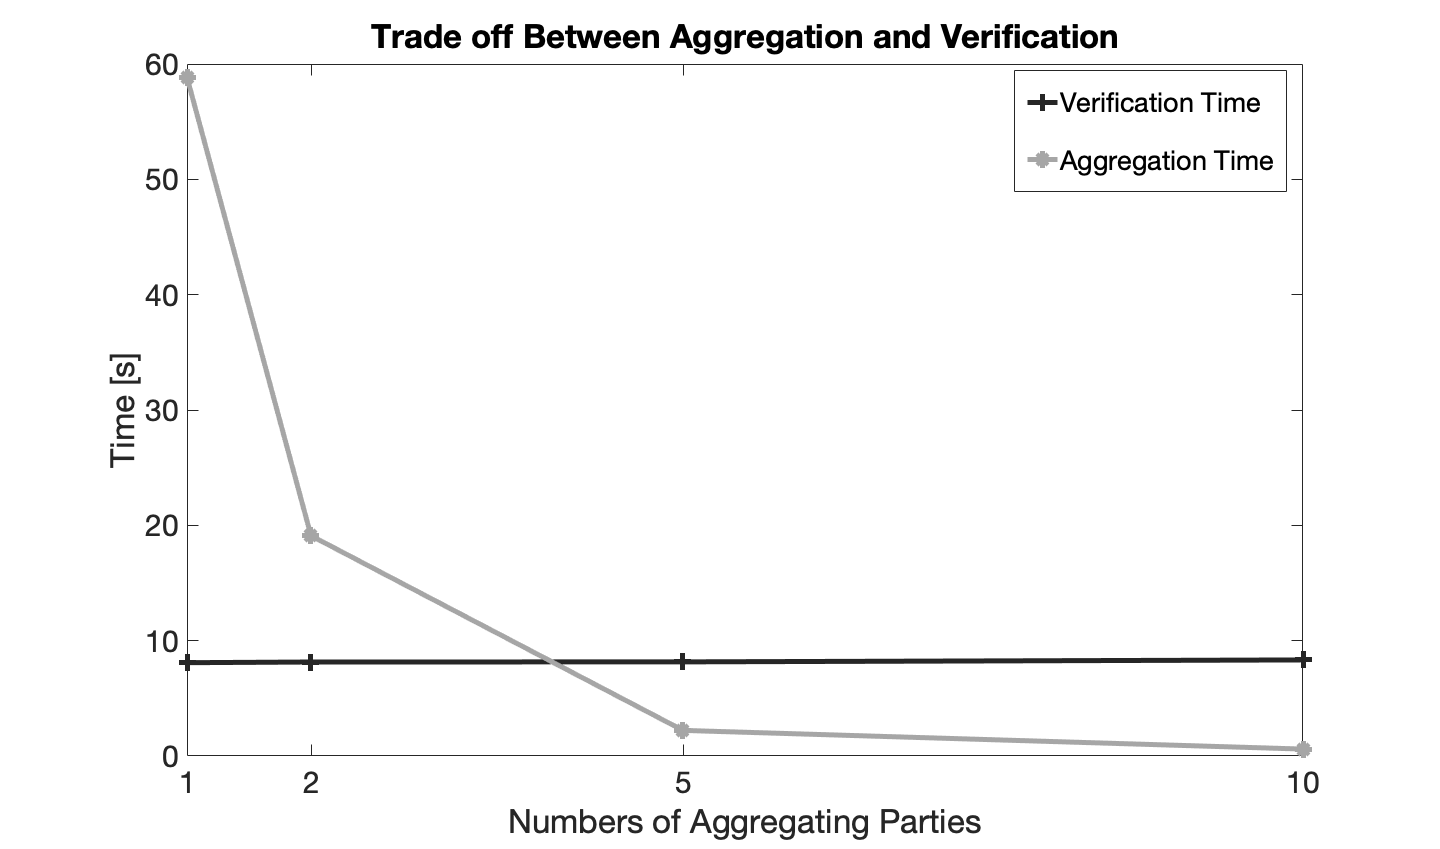
\includegraphics[width=\linewidth]{./figure/trade-off.png}
\caption{Timing in seconds for running the algorithms  \textbf{Aggregate} and \textbf{Verify} in Construction \ref{alg:ZKSM-Agg-Many} considering different numbers of aggregating parties. The number of aggregating parties varies between $1,2,5$ and $10$. The figure is a visualisation of the results presented in Table \ref{tab:tradeoff}. }
\label{fig:tradeoff}
\end{figure}

Figure \ref{fig:tradeoff}, which is a visualisation of the values in Table \ref{tab:tradeoff},  shows that if the aggregation is shared between a set of aggregating parties the runtime per aggregating party is reduced almost exponentially. At the same time the increased runtime for verifying multiple aggregated proofs is linear. Resulting in that splitting the aggregation between a set of aggregating parties reduced the total runtime for the construction and per aggregating party.



\begin{table}
\centering
\caption{Timing in seconds for algorithms  \textbf{Aggregate} and \textbf{Verify} in Construction \ref{alg:ZKSM-Agg-Many} considering different numbers of aggregating parties, $|\mathcal{K}|$.
 }
\begin{tabular}{c | c c}
\toprule
$|\mathcal{K}|$ &  \textbf{Aggregate} [s] & \textbf{Verify} [s]\\	\midrule
  1					 							&   58.84 	&	8.09\\ 
  2												&   19.10 	&	8.15\\ 
  5												&   2.22 	& 8.16\\
  10												&   0.60 	& 8.33\\ \cdashline{1-3}
  Not aggregated												&   -	& 9.29\\ 
  \bottomrule 
\end{tabular}
 \label{tab:tradeoff}
\end{table}



% 20 procnt speed up by aggrgegating. 
%The aggregated version of the set membership and signature-based range proof has not been implemented thus result about how this aggregation affects the runtime can not be determined. In order to still get some idea of the runtime reduction, the algorithm \textbf{Verify} in Construction \ref{alg:ZKSM} was reduced to: 
%\begin{itemize}
%\item\text{\textbf{Verify} $(g,h,C,\textit{proof})\xrightarrow[]{}\{0,1\}$}
%Check if $a \overset{?}{=} e(V,y)^c e(V,g)^{-z_x}e(g,g)^{z_\tau}$. If the equality holds the prover has convinced the verifier that $x\in\Phi$ return $1$ otherwise return $0$.
%\end{itemize}
%Then the runtime of this algorithm ran $100$ times, once for each clinet, was compared to the original version ran $100$ times. This gave the result that the modified version was approximately $20\%$ faster. This given some indication of the speed up obtained by aggregating since the equality check $D\overset{?}{=} C^ch^{z_\tau}g^{z_x}$ will only have to be ran once thus this runtime might be ignored in the context. 

\section{Comparison to Bulletproofs}
\label{sec:ComparetOBullet}
In this section, the construction of aggregated signature-based set membership proofs are compared to the state-of-the-art Bulletproofs. The focus of comparison is the runtime of a party verifying of multiple proving parties. In this section the aggregation is considered to be performed by a single party, i.e $|\mathcal{K}|=1$. Before presenting the results, Bulletproofs are described in more detail.

\subsection*{Bulleproofs settings}
% Regarding aggregation of Bulletproos
The original paper about Bulletproofs \cite{bulletProofs_theory} presents a method for aggregating Bulletproofs such that $n$ parties, each having committed to a Pedersen commitment, can generate a single Bulletproof verifying that each commitment hides a secret in an allowed range. The proposed method for aggregation is an interactive construction, since it is required that all provers construct their proofs using for the same challenges. If the provers were to use different challenges the verification would fail.

To Conclude, Bulletproofs can be aggregated with the cost of an interactive construction. Since this paper aims to investigate non-interactive constructions,  non aggregated Bulletproofs are considered. Therefore the verifier has to verify all Bulletproofs separately, i.e once for each prover. 
%Regadring compelxity depending on n in Bulletproofs

The computational complexity for verification of a Bulletproof depends on the maximum upper bound of the range, i.e it depends on $n$ determining the range $[0,2^n)$. This motivates to see how the runtime is affected by considering different maximal upper bounds.  The maximal upper bound of Bulletproofs is $2^n$, for some $n$ that is a power of $2$. Two different values of $n$ are considered for comparison $n=8 $ and $n=32$. 

Bulletproofs can be modified to allow arbitrary ranges $[a,b]$, such that $b<2^n$ and $a<b$ , with the same approach as presented for the signature-based range proofs and illustrated in Figure \ref{fig:interval}. This is exploited and the range is set to $[18,200]$. 

 
 %, however this is not a desirable property for the the server and client verifiable AHSS. Investigation about whether this construction can be modified to be completely non-interactive has not been done and remains an open question.  

%This concludes that neither of the considered range proofs has be sucessfully fully aggregated aggregated  such that the verifier can perform one single verification instead of one for each client, at least not without some cost. Remark that this conclusion is not final and their may very well exist small or large modifications of the range proof that will allow them to be aggregated and still remaining non-interactive. The investigation of such modification is outside the scope of this paper but the reader is endorsed to explore this possibility. 

%Uniformly for Bulletproofs, signature-based range poofs and set membership proofs the runtime for \textbf{VerifyRP} is longer then \textbf{VerifyServers}. This is despite the fact that \textbf{VerifyRP} corresponds to the runtime of verifying one clients while \textbf{VerifyServers} is the runtime to verify all severs. This highlights how expensive the verification of clients are and motivates the  attempts to aggregate the verification of clients. 

\subsection*{Runtime Comparison}
This section will compare runtime results considering the verification of $100$ proofs using Bulletproofs and aggregated signature-based set membership proofs.  Bulletproofs with an upper bound equal to $2^8$ and $2^{32}$ are considered meaning that in total three constructions are compared.

A remark is that the computational complexity of Bulletproofs depend on the variable $n$, where $n$ determines the maximal upper bound of the range. The signature-based set membership proofs have a computational complexity of $\mathcal{O}(1)$ for the proof construction and verification, meaning that the complexity is independent of the size of the set $\Phi$. Therefore, to provide a comparison between Bulletproofs and aggregated signature-based set membership proofs considering different applications scenarios,  the runtime for verification of Bulletproofs is presented considering two different values of $n$.

Table \ref{tab:CompareToBulletproof} shows the runtime for the verification of $100$ proofs using the three considered constructions.

\begin{table}
\centering
\caption{Runtime for verification of $100$ proofs constructed using three different ZKP. The three considered proof constructions are: Bulletproofs, with a maximal upper bound equal to $2^8$ and $2^{32}$, and aggregated signature-based set membership proofs. }
\begin{tabular}{l | r }
\toprule
	  											& \textbf{Verify} [s]\\	\midrule
  Bulletproofs, $n=8$					&   2.98 		\\ 
  Bulletproofs, $n=32$					&   10.22 		\\ 
  Aggregated Set Membership Proofs 	&   8.09 	 \\ 
  \bottomrule 
\end{tabular}
\label{tab:CompareToBulletproof}
\end{table}

Bulletproofs with an upper bound equal to $2^8$ is considerably faster than the other constructions, however, it is highly limited in its applications since the upper bound is fairly low. The runtime for Bulletproof with an upper bound equal to $2^{32}$ is longer than for aggregated set membership proofs. Thus, aggregated signature-based set membership proofs is a relatively fast and yet flexible implementation. 

In Figure \ref{fig:NrClients} the runtime for verification is given as a function of the number of provers. In addition to the above constructions, signature-based set membership proofs are considered. The runtime has been measured considering  $1,25,50,75,100,125$ and $150$ provers respectively.  From the figure, it is seen that there is a linear relationship between the number of provers and the runtime for verification. It is also seen that the runtime relationship between the different constructions seen in Table \ref{tab:CompareToBulletproof}, appears to remain independent of the number of provers. 

In Figure \ref{fig:NrClients} it is noted that the difference between the runtime for the aggregated signature-based set membership proof and the ordinary signature-based set membership proofs, increases with the number of provers. This result is expected since the difference in the number of computation performed by the verifier increases linearly with the number of provers. 

To conclude, whether Bulletproofs or aggregated signature-based set membership proofs are faster in terms of runtime for the verifier depends on the application, since the runtime for verifying  Bulletproofs depends on the maximal upper bound of the range. The rule of thumb is that aggregated signature-based set membership proofs are faster when considering a large range and Bulletproofs are faster when considering a small range. It is however always true that set membership proofs are more flexible than range proofs since they allow non-continuous discrete sets. An important thing to mention, although not the focus of this comparison, is that the set-up phase of aggregated signature-based set membership proofs is linear in the number of elements in the set, resulting in that it is computationally demanding for large sets. 


%TODO deside if use this, plus rerun all values!
% The Bulletproofs has computational complexity $\mathcal{O}(log_2 n)$, thus an expected increase of a factor $5/3\:(=log_2\: 32/ log_2\: 8)$ would be expected, however in Figure \ref{fig:NrClients} an increase of a factor approximately $4$ is seen for the algorithm \texttt{Verify} in Construction \ref{alg:VAHSS-HSS-RP} when increasing $n$ form $8$ to $32$, why this result is obtained is not clear.


 \begin{figure}[]
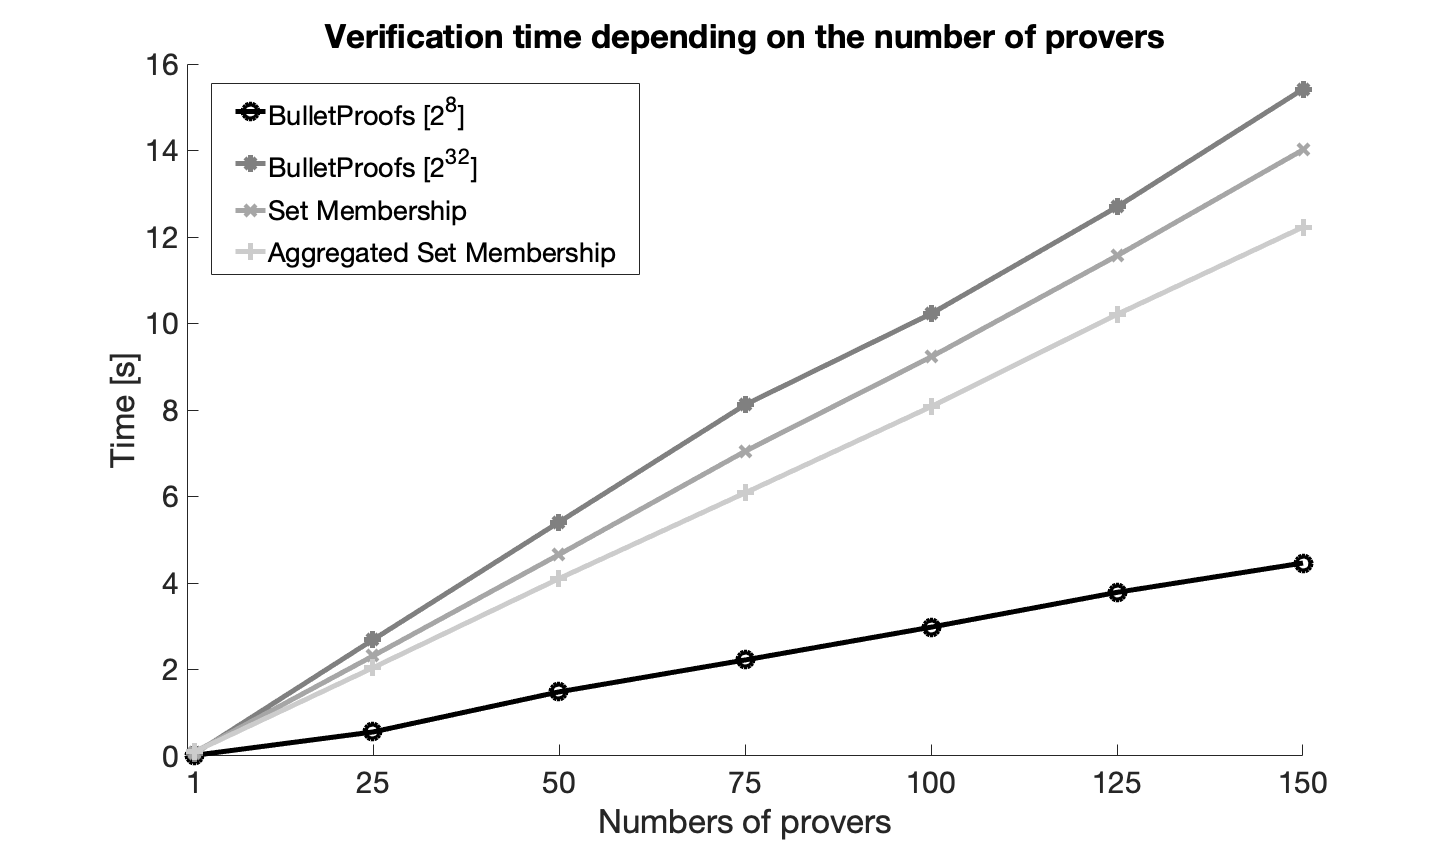
\includegraphics[width=\linewidth]{./figure/verificationNbrClients.png}
\caption{Runtime for verification of multiple provers as a function of the number of provers. Verification of four different constructions of proofs  are considered: aggregated signature-based set membership proofs, signature-based set membership proofs, Bulletproofs with a maximal upper bound equal to $2^8$ and Bulletproofs with a maximal upper bound equal  to $2^{32}$.}
\label{fig:NrClients}
\end{figure}
